\documentclass[12pt,letterpaper]{article}
\usepackage{fullpage}
\usepackage[top=2cm, bottom=4.5cm, left=2.5cm, right=2.5cm]{geometry}
\usepackage{amsmath,amsthm,amsfonts,amssymb,amscd}
\usepackage{lastpage}
\usepackage{enumerate}
\usepackage{fancyhdr}
\usepackage{mathrsfs}
\usepackage{graphicx}
\usepackage{hyperref}
\usepackage{wrapfig}
\setlength{\parindent}{0.0in}
\setlength{\parskip}{0.05in}

% Edit these as appropriate
\newcommand\course{CS1420}
\newcommand\semester{Spring 2026}          % <-- current semester
\newcommand\hwnumber{4}                    % <-- homework number

\pagestyle{fancyplain}
\headheight 35pt
\chead{\textbf{\Large Homework Report \hwnumber}}
\rhead{\course\;--\;\semester \\ \today}
\lfoot{}
\cfoot{}
\rfoot{\small\thepage}
\headsep 1.5em

\begin{document}

\section*{Part a}

To learn the model weights, binary logistic regression is implemented using mini-batch stochastic gradient descent. The model uses the sigmoid function to predict the probability that an observation belongs to class 1: $h_{\mathbf{w}}(\mathbf{x})=\frac{1}{1+e^{-\mathbf{w}^T\mathbf{x}}}$.

The original binary cross-entropy loss is $L(\mathbf{w})=-\frac{1}{m}\sum_{i=1}^{m}\left[y_i\log h_{\mathbf{w}}(\mathbf{x}i)+(1-y_i)\log(1-h{\mathbf{w}}(\mathbf{x}_i))\right]$.

Then we incorporate L2 regularization by adding a penalty proportional to the sum of squared weights $L_{\mathrm{reg}}(\mathbf{w})=L(\mathbf{w})+\lambda|\mathbf{w}|_2^2$, where the larger the weight is, the larger the penalty will be.

Then we take the derivative, the gradient for each mini-batch will be 

\[
\nabla L_{\mathrm{reg}}(\mathbf{w})=
\frac{1}{m}X^T(h_{\mathbf{w}}(X)-Y)+2\lambda\mathbf{w},
\]
where $m$ is the number of samples in the current mini-batch.

The weights is updated using $\mathbf{w}_{new}\leftarrow\mathbf{w}_{old}-\alpha\nabla L_{\mathrm{reg}}(\mathbf{w})$ where $\alpha$ is the learning rate. For each epoch, the training examples were shuffled and divided into mini-batches. The weights were updated using the gradient calculated from each batch. The term $2\lambda\mathbf{w}$ penalizes large weights, which helps prevent the model from overfitting.


\section*{Part b}

Without L2 Tikhonov regularization $\lambda=0$, the model would minimize only the binary cross-entropy loss. In terms of that, larger weights will be assigned to individual features to fit the training data more closely.

Unregularized model usually contains additional features that may not be informative so that it could overfit the training data, resulting in a larger gap between training and validation accuracy. By applying L2 regularization, we can constrain the magnitude of the weights and reduce the model's sensitivity to noise. This can improve generalization and reduce validation error. However, excessive regularization may cause underfitting, which case is shown in the result of our trained model in part c, increasing both training and validation errors.

When considering classification errors, regularization can affect both false positives (i.e. a patient without cancer is classified as having cancer) and false negatives (a patient with cancer is classified as not having cancer). Regularization does not necessarily reduce both types of errors, and its effect depends on the dataset and decision boundary.


\section*{Part c}

\begin{figure}
    \centering
    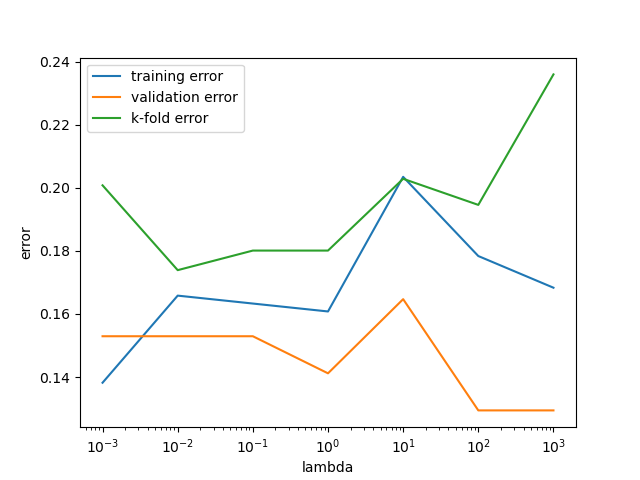
\includegraphics[width=0.75\linewidth]{Figure_1_Lambda_1.png}
    \caption{Model selection curve with $\Delta$ of $\lambda$}
    \label{fig:placeholder}
\end{figure}

7 regularization parameters, $\lambda \in \{0.001, 0.01, 0.1, 1, 10, 100, 1000\}$, were evaluated using training error, validation error, and 3-fold cross-validation error. The results are shown in the model selection plot (Fig. 1).

Based on the graph as shown above in Figure 1, $\lambda=1$ is chosen as the optimal regularization parameter with the training error around $16\%$ and the validation error around $14\%$ where k-fold validation error is around $18\%$. The model achieved relatively low errors across all three evaluations.

Although some other lambda values achieved lower errors on individual evaluation metrics, $\lambda=1$ provided a reasonable balance between training performance and generalization. Smaller lambda values allow more flexibility in fitting the training data, potentially increasing the risk of overfitting (i.e. $\lambda=0.001$ with a big gap in training and k-fold error), while larger lambda values impose stronger penalties on the weights and may lead to underfitting (i.e. $\lambda=1000$ with very high k-fold error).


\section*{Part d}

Yes, we definetely need to account for the situations when multiple samples were collected from one patient. We need to group the samples from one patient first and then split each group samples as a intact set into either training or test or validation set. The same patient-level grouping should also be maintained during k-fold cross-validation. If samples from one patient appeared in both the training and validation or test sets, the model could learn patient-specific patterns, leading to data leakage and thus overfitting and causing worse generalization to outside dataset.


\end{document}